\section{力的单位}\label{sec:2-3}

力是有大小的。大人能提起一大桶水,小孩只能提起一小桶水,这是因为大人的力气比小孩的力气大。
从生活经验中我们还知道,拖拉机的拉力比牛的拉力大,机车的拉力比汽车的拉力大。

为了测量力的大小,必须确定力的单位。在国际单位制中,力的单位是\textbf{牛顿}\footnotemark。
牛顿这个单位是怎样规定的,我们到高中再学习,现在只需要知道,\textbf{质量为 $1$ 千克的物体受到的重力是 $9.8$ 牛顿}。
在今后学习中,我们将主要用牛顿作力的单位。
\footnotetext{在物学中,有许多物理量的单位是用科学家的名字命名的。力的单位牛顿就是用英国科学家牛顿的名字命名的。}

为了表示质量为 1 千克的物体受到的重力是 $9.8$ 牛顿,物理学中把这个意思写作“$9.8$ 牛顿/千克”。
读作 “$9.8$ 牛顿每千克”\footnotemark,并且用字母 $g$ 来代表,即
\footnotetext{物理量单位中的斜线读作“每”, 斜线表示除的意思。
在后面的学习中可以看到,两个量相乘或者相除时,它们的单位也相乘或者相除;
在单位乘、除的过程中,分子和分母中同名单位要约去,这跟分式运算中分子和分母的公因式要约去一样。}


\centerline{$g = 9.8$ 牛顿/千克。}

因为物体受到的重力跟它的质量成正比,所以知道了 1 千克物体重 $9.8$ 牛顿,就可以算出
$2$ 千克物体重是 $2\text{千克} \times 9.8 \text{牛顿/千克} = 19.6 \text{牛顿}$,
$3$ 千克物体重是 $3\text{千克} \times 9.8 \text{牛顿/千克} = 29.4 \text{牛顿}$,
$m$ 千克物体重是 $m\text{千克} \times 9.8 \text{牛顿/千克}$。
因此,物体所受的重力跟质量的关系式是

\centerline{$\text{重力} = \text{质量} \times 9.8 \text{牛顿/千克}$。}

\begin{wrapfigure}[10]{r}{5cm}
    \centering
    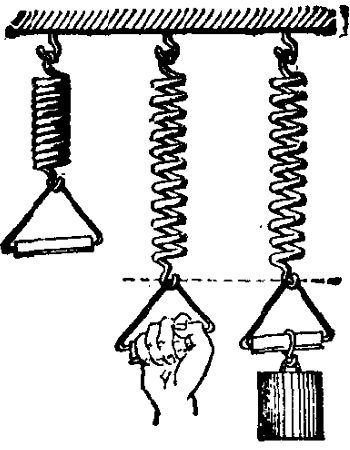
\includegraphics[width=0.2\textwidth]{../pic/czwl1-ch2-6}
    \caption{手的拉力跟钩码所受的重力相等}\label{fig:2-6}
\end{wrapfigure}


如果用 $G$ 代表重力, $m$ 代表质量, $g$ 代表 $9.8$ 牛顿/千克,那么上面的关系式可以写作

\centerline{$G = mg$。}

在用上面的公式计算重力时,质量 $m$ 的单位一定要用千克,计算出的重力单位才是牛顿。

知道了重力的大小, 我们就可以用它来测量其它力的大小。例如,如果我们用手把弹簧拉到某一长度,
而用重 50 牛顿的钩码也能够把弹簧拉到同一长度,那么手的拉力就等于钩码所受的重力,即 50 牛顿(图 \ref{fig:2-6})。

牛顿这个单位是比较小的。我们的这本物理课本重大约就是 1 牛顿,成年人的体重一般是 500 ~ 700 牛顿,蒸汽机车的牵引力有十几到二十几万牛顿。
\footnote{在实际中,还常用千克力作力的单位。1 千克力是质量 1 千克的物体所受的重力。因此,$1 \text{千克力} =  9.8 \text{牛顿}$。}

\lianxi

(1) 某同学的质量是 50 千克,他体重是多少牛顿?

(2) 搬起一块质量为 25 千克的石头,至少需要多少牛顿的力?

(3) 某举重运动员能举起 170 千克的杠铃,他能不能举起重 1500 牛顿的一块钢锭?

(4)\mylabel{shiyong-keben-zhiliang} 根据前面称出的\hyperref[celiang-keben-zhiliang]{物理课本的质量},算出它重多少牛顿。
用手掂一掂课本,再掂一掂铅笔盒和一杯水,估计出铅笔盒和这杯水重多少牛顿。


